\section{Materials and methods}
\label{p3:sec:methods}

\subsection{Participants}

Eight naive participants (three male, five female), aged between 22 and 29 years, provided written informed consent to participate in the experiment. All participants were free of any known vestibular or neurological disorder and had normal or corrected-to-normal visual acuity. Participants never received any feedback about their performance.

\subsection{Experimental setup}

A motorized linear sled \cite<see>[for details]{clemens2012} was used to laterally translate participants following a minimum jerk profile \cite{flash1985} of fixed duration (1 \si{\second}) and amplitudes ranging from 1 to 27 \si{\centi\metre}. Participants were seated on the sled such that the inter-aural axis aligned with the motion axis. They were restrained using a five-point seat belt and a chin rest. In addition, the head was held in place using a sled-fixed mold which resembled head-phones and pressed down on the head surrounding the pinnea . Auditory cues were suppressed using white noise presented through in-ear headphones. Experiments were conducted in complete darkness except for visual fixation points, projected by a laser pointer on a black bar 50 \si{\centi\metre} in front of the participant at eye level. Laser pointers used to project body-fixed targets were attached to the sled. Those used to project world-fixed targets were mounted on the wall behind the sled.

Eye movements were recorded at 500\si{\hertz} using an EyeLink II (SR Research, Kanata, Canada) system whose cameras were mounted to the sled and therefore remained stable with respect to the head during the entire experiment. Because the head and body positions were fixed during the experiment, the orientation of the eyes within the head, as measured by the tracker, was equivalent to the orientation of the eyes in space. The eye tracking system was calibrated before each session using 11 evenly spaced calibration points ranging from -22 to \siang{22} degrees. We used linear regression to link EyeLink measurements to gaze angles.

\subsection{Paradigm}
We used a two-alternative forced choice (2-AFC) task to measure perceived linear self-motion across three different eye fixation types: world-fixed, body-fixed, and unconstrained (free) fixation. We refer to these as world, body and free, respectively. A trial contained two sequential translation intervals of equal duration (1 \si{\second}) and in the same direction (either leftward or rightward). Different fixation types were presented in the two translation intervals. Participants were instructed to judge whether the translation during the second interval was longer or shorter compared to the first interval. They were additionally instructed to always look at the fixation point when it was visible; no instructions were given for when the fixation point was switched off (i.e. during free fixation).


\begin{figure}
    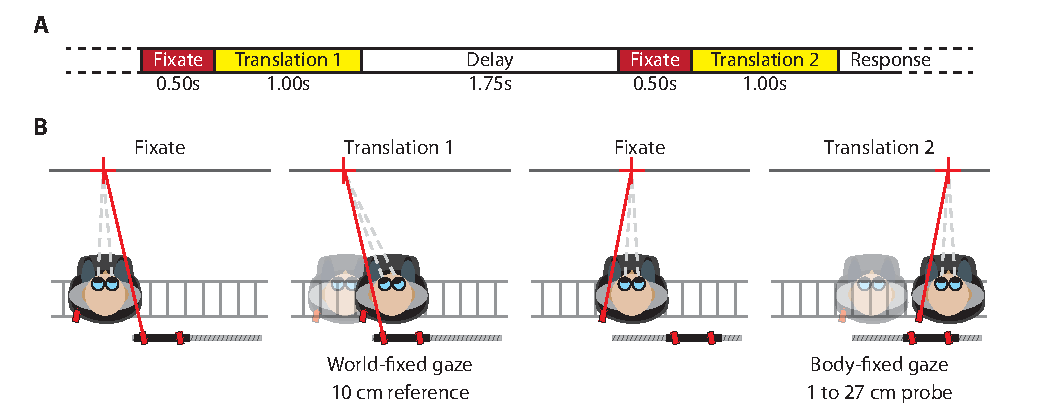
\includegraphics[width=1.0\textwidth]{src/paper3/figure1.pdf}

    \caption{\panelref{A} Time course of key events within a single trial. In each of the two intervals, a 0.50 \si{\second} fixation period (red) precedes the lateral translation (yellow). A 1.75 \si{\second} long delay period (shown in white) separates the two intervals. After the second translation, the participant responded whether this second translation was longer or shorter than the first. \panelref{B} Top-view illustrating key events during a body vs. world trial. First panel: participant fixates the world-fixed target (red cross) at the start of the first interval. Second panel: translation with world-fixed fixation target. Third panel: body-fixed fixation at start of second fixation interval. Fourth panel: translation with body-fixed fixation in second interval.}
    \label{p3:fig1}
\end{figure}

The time evolution of a single trial is shown in \figref{p3:fig1}. Each trial started with the onset of a central fixation point (i.e. aligned between the eyes) for 0.5 \si{\second}. Subsequently, the first translation interval commenced.  Depending on the fixation type, the fixation point remained visible (world and body) or was extinguished (free) during the translation interval. The trial shown in the figure depicts the 10 \si{\centi\metre} reference translation with world fixation. After this first interval, a delay followed in which the participant was kept in complete darkness for 1.75 \si{\second}. Then, the central fixation point reappeared, followed 0.5 \si{\second} later by the second interval, in which the probe translation was presented. The set of possible probe translations ranged from 1 to 27 \si{\centi\metre} in equidistant steps of 0.4 \si{\milli\metre}. The fixation type in the probe interval was always different than in the associated reference interval (the trial in \figref{p3:fig1} illustrates body fixation). After the second interval, the participant had to indicate whether he or she perceived the second translation as longer or shorter than the first using a 1-dimensional joystick. Moving the poke away from the body indicted that the second movement was longer, while moving it towards the body indicated that the second movement was shorter.


\begin{table}
    \begin{tabular}{llll}
    Comparison & Reference & 1st interval & Direction \\
    \hline
    Body vs. world & Body & Reference & Right \\
    & & & Left \\
    & & Probe & Right \\
    & & & Left \\
    \cline{2-4}
	& Body & Reference & Right \\
    & & & Left \\
    & & Probe & Right \\
    & & & Left \\
    \hline
    Body vs. free & Body & Reference & Right \\
    & & & Left \\
    & & Probe & Right \\
    & & & Left \\
    \cline{2-4}
	& Free & Reference & Right \\
    & & & Left \\
    & & Probe & Right \\
    & & & Left \\
    \hline
    World vs. free & World & Reference & Right \\
    & & & Left \\
    & & Probe & Right \\
    & & & Left \\
    \cline{2-4}
	& Free & Reference & Right \\
    & & & Left \\
    & & Probe & Right \\
    & & & Left \\
    \end{tabular}

    \caption{List of the three main comparisons that we tested. The (10 \si{\centi\metre}) reference movement was presented in either the first or second movement interval. We also manipulated movement direction (leftwards or rightwards), yielding a total of 24 trial types.}

    \label{p3:tab1}
\end{table}

Thus, a trial consists of two translations with different fixation types; in the three main conditions we compare the body versus world, world versus free, and body versus free fixation types. For each main condition, we varied which fixation type served as the reference stimulus and the order in which reference and probe were presented, which gives a total of four variations per main condition (see \tabref{p3:tab1}). In addition we varied translation direction (either leftward or rightward on consecutive trials). The amplitude of the probe translation was adaptively chosen using the Psi method. This method picks the amplitude for the next trial which maximizes the expected decrease in entropy based on participants’ responses to earlier trials \cite{kontsevich1999}. This was done separately for all 24 trial types (3 main conditions x 2 reference stimuli x 2 reference/probe orders x 2 translation directions; see \tabref{p3:tab1}). A total of 25 trials were collected per trial type yielding a total of 200 trials for each of the three main conditions.

Trials were presented in three one-hour sessions. To prevent dark adaptation, we turned on the lights for 5 \si{\second} after every block of 6 trials, and for at least 30 seconds every 4 blocks. We made sure that each of the 24 unique trial types were presented once every 4 blocks. After each block, the adaptive procedure determined which translation amplitudes to test in the following block. To increase the number of data-points available to the adaptive psychometric procedure at the beginning of the experiment, we collapsed across translation direction and reference order for the first 10 trials of every condition. After those collapsed trials, the procedure ran separately for each of the 24 distinct trial types.

\subsection{Data analysis}

For each combination of the three main conditions, and  the two reference/probe orders (see \tabref{p3:tab1}), we quantified the perceived probe translation  by calculating the probability of the probe translation judged longer compared to the 10 \si{\centi\metre} reference translation as a function of actual probe translation, given by x. We used a maximum likelihood fit of a cumulative Gaussian function to summarize the psychometric data:

\begin{equation}
\label{p3:eq1}
P(x) = \lambda + (1 - 2\lambda) \frac{1}{\sigma \sqrt{2\pi}} \int_{-\infty}^{x}{e^{-(y-\mu)^2 / 2\sigma^2}}dy,
\end{equation}

in which $|x|$ represents the size of the absolute probe displacement. The mean of the Gaussian represents the point of subjective equality (PSE). The slope of the curve reflects the precision ($1/\sigma$) of reference-probe discrimination performance. Parameter $\lambda$, representing the lapse rate, accounts for stimulus-independent errors caused by subject lapses or mistakes and was restricted to small values ($\lambda < 0.06$. Fits were performed using the Psignifit toolbox \cite{wichmann2001,wichmann2001b}.

For each trial type (see \tabref{p3:tab1}), we also qualified eye movements, corrected for drift, based on initial fixation. The main source of drift were tiny lateral movements of the eye tracking cameras due to sled motion. We discarded trials containing blinks as well as trials in which the final eye position exceeded two standard deviations from the condition's average. Based on these criteria, 6.1\%, 3.6\% and 1.6\% of all trials were rejected based on errors in body, world, and free fixation respectively. In addition we rejected 1.2\% of all trials because participants blinked within the movement interval.

For the remaining trials, we computed the average ratio between the measured eye excursion, $\varphi_i$, and the angle that woud be needed were the trial testing the world-fixed condition. The latter is computed by taking the arc-tangent of the actual translation distance, $m_i$, divided by the fixation depth, $d_i$, which for small $\varphi$ can be approximated by $g = \varphi m/d$. We computed this ratio, $g$, for every fixation type and interval (see \tabref{p3:tab1}). Ideally, for body-fixed trials $g = 0$, and for world-fixed trials $g = 1$. Using this ratio, we are able to compute the expected eye excursion, $\hat{\varphi} = gd/m$, for any given translation distance even those we did not explicitly measure.

\subsubsection{Model}

Using a simple cue integration model, we investigated whether inter-subject and inter-condition differences in the observed PSEs in conditions containing a translation under free fixation depend on actual eye movement behavior. We modeled perceived distance, $p$, as a weighted linear combination of a vestibular and an oculomotor estimate of translation (\eqnref{p3:eq2}). We assumed that the vestibular estimate is equal to the actual translation, $m$, and that the oculomotor estimate is equal to expected eye movement given the  actual, $\hat{\varphi}_{m_i}$. As the weights represent the relative contributions of the oculomotor and vestibular systems, they can sum to any arbitrary value; in \eqnref{p3:eq2} they are fixed to 1. Thus, the weighting parameter $\alpha$ regulates the eye movement contribution and $1 - \alpha$  the vestibular contribution:

\begin{equation}
\label{p3:eq2}
p = \alpha \hat{\varphi}_m d + (1 - \alpha) m = \alpha g m + (1 - \alpha) m
\end{equation}

By definition, the probe displacement is perceived as equal in length to the 10 \si{\centi\metre} reference displacement at the PSE. By substituting both sides by the right hand side of \eqnref{p3:eq3} and using subscripts for reference ($r$) and probe intervals ($p$), we obtain:

\begin{equation}
\label{p3:eq3}
\alpha g_r m_r + (1 - \alpha) m_r = \alpha  g_p m_p \alpha + (1 - \alpha) m_p + \epsilon
\end{equation}

In the present experiment, the reference displacement, $m_r$, was always 10 \si{\centi\metre} and the probe displacement, $m_p$, was equal to the measured PSE for the presented combination of fixation types (i.e, $PSE$ in \eqnref{p3:eq1}). This model (i.e. \eqnref{p3:eq3}) was then fit to data from the body and world conditions using linear regression, finding weight α that minimizes the sum of squared errors ($\sum{\epsilon^2}$).

\begin{equation}
\label{p3:eq4}
m_r - m_p = \alpha(g_{f_p} m_p - g_{f_r} m_r + m_r - m_p) + \epsilon
\end{equation}

By only using data from conditions where a visual fixation point was present (i.e. body versus world) to fit the model, we examined if the same weight $\alpha$ also explains the PSEs found in the conditions where fixation was free. To this end, we solved Equation 3 for $m_p$ and computed PSE estimates, $P\hat{S}E$, for the body versus free and world versus free conditions (\eqnref{p3:eq5}).
                                                                                            \begin{equation}
\label{p3:eq5}
\hat{m}_p = P\hat{S}E = \frac
	{\alpha g_r + (1 - \alpha)}
	{\alpha g_p + (1 - \alpha)}
    m_r
\end{equation}

In addition to minimizing the sum of squared errors in \eqnref{p3:eq4}, we also fit \eqnref{p3:eq5} to the data in order to see if weight α depends on the way the model is formulated. Parameters obtained by fitting \eqnref{p3:eq5} fell well within the standard deviation reported in \tabref{p3:tab2} for all participants, suggesting that they did not depend on the way the model was formulated.
